\documentclass[10pt, a4paper]{article}
\usepackage{ictam}
\usepackage[sort&compress]{natbib}
\usepackage{amsmath}
\usepackage[utf8]{inputenc}
\usepackage[english]{babel}
\usepackage{amssymb}
\usepackage{graphicx}
\usepackage{amsthm}
\usepackage{makecell}
\usepackage{wrapfig}
\usepackage[T1]{fontenc}
\usepackage[utf8]{inputenc}
\usepackage[font=small,labelfont=bf]{caption}
\usepackage[demo]{graphicx}
\usepackage{booktabs}
\usepackage{calc}
\usepackage{lipsum}

\begin{document}

\title{Input-output inspired method for bounding permissible perturbation amplitude: application to a transitional shear flow model}

\author[1]{\underline{Chang Liu}{\footnote{Corresponding author. E-mail: changliu@jhu.edu}}}
\author[1]{{Dennice F. Gayme}} 
%Corresponding author email should be added like this
\affil[1]{Department of Mechanical Engineering, Johns Hopkins University, Baltimore, U.S.A.}
%\affil[2]{Department of Another Author, University of Another Author, City, Country}

\maketitle
\vspace{-3mm}

\begin{abstract}
Determining the permissible level of perturbation to maintain a laminar flow state is of critical importance in a wide range of applications. Historical approaches to this problem in wall-bounded shear flows focused on linear analysis that is only provably valid in a small neighborhood of the laminar solution and preclude the evaluation of the role of nonlinearity. Extensive simulations or experimental studies allow exploration of the full dynamics, but a finite set cannot provide a definitive bound. This work takes an input-output approach to construct a model of the nonlinear term that is constrained by system physics to be energy conserving (passive) and to have bounded input-output energy in a local region. This model allows a more computationally efficient solution than prevailing nonlinear approaches based on Sum of Squares (SOS) programming. We apply our approach to a low dimensional nonlinear shear flow model for a range of Reynolds numbers. The results from our analytically derived bounds are consistent with the bounds identified through exhaustive simulations. However, our results are obtained at a much lower computational cost and have the benefit of providing a provable guarantee that a certain level of perturbation is permissible.
\end{abstract}

\vspace{-6mm}
\section{INTRODUCTION}
\label{sec:introduction}
\vspace{-2mm}

%; e.g., Rayleigh Bernard instability \citep{koschmieder1993benard}.
The critical Reynolds number $Re_C$ of transition to turbulence in wall-bounded shear flows is typically not equal to that predicted by linear stability analysis; i.e., $Re_L\neq Re_c$. This mismatch may be attributed to the failure of the infinitesimal perturbation assumption in the linear stability analysis due to the transient growth \citep{henningson1994role}. The energy stability method \citep{joseph2013stability} allows us to determine the Reynolds number $Re_E$ below in which the base flow is stable against any finite perturbation, but the predicted $Re_E$ is typically too conservative; i.e., $Re_E<Re_C$. In the range $Re_E<Re<Re_L$, there exists a permissible level of perturbation to maintain a laminar flow state, which is of critical importance in understanding transition to turbulence and flow control applications. However, a finite set of experiments or numerical simulations in a finite time interval cannot provide a definitive bound of the permissible level of perturbation to maintain a laminar flow state. This work constructs a model of the nonlinear term that is constrained by system physics to be energy conserving and to have bounded input-output energy in a local region, specifically focusing on determining the critical perturbation amplitude in a computationally efficient manner. 

%Based on Lyapunov' method for stability, we formulate the critical perturbation amplitude problem  into a Linear Matrix Inequality (LMI) \citep{boyd1994linear} and use the available solver such as YAMLIP \citep{lofberg2004yalmip} to solve the problem efficiently.

%With obtained permissible perturbation amplitude, we compare its Reynolds number trends with that reported in the literature \citep{baggett1997low,Joglekar2015} and further compare the results and computational resources with the Sum of Squares method. The resulting critical perturbation amplitude is conservative, yet consistent, compared with that estimated from simulations \citep{baggett1997low,Joglekar2015} with randomly chosen initial conditions. Compared with the Sum of Squares approach, the proposed framework is more computationally efficient as we describe the nonlinearity as the input-output property explicitly instead of automatically exploring the property of nonlinearity yet implicitly. 

\vspace{-2mm}

\section{INPUT-OUTPUT DESCRIPTION OF NONLINEARITY}
\vspace{-2mm}

For a shear flow model with state variable $\boldsymbol{a}\in\mathbb{R}^n$, we partition the underlying dynamics as: $\frac{d\boldsymbol{a}}{dt}=\boldsymbol{L}\boldsymbol{a}+\boldsymbol{f}$, where the equilibrium point of interest is shifted to the origin. The $\boldsymbol{L}\in\mathbb{R}^{n\times n}$ represents the linear components of the dynamical system, and the term $\boldsymbol{f}\in\mathbb{R}^n$ represents the remaining nonlinear components, which is written as $ \boldsymbol{f}=\boldsymbol{J}(\boldsymbol{a})\boldsymbol{a}$ and viewed as the feedback forcing of the linear system. Using certain input-output properties between the input $\boldsymbol{f}$ and output $\boldsymbol{a}$, nonlinearity can be taken into account in stability analysis. For example, the input-output property $\boldsymbol{a}^T\boldsymbol{M}_0\boldsymbol{f}=0$ with $\boldsymbol{M}_0=\boldsymbol{I}$ can describe the energy conserving property of nonlinear term and reproduce the same requirement of energy stability \citep{goulart2012global}. Here, we explore more input-output properties for the nonlinear term $\boldsymbol{f}$ such as a non-trivial $\boldsymbol{n}$ satisfying $\boldsymbol{n}^T\boldsymbol{f}=0$, which is described as the input-output properties: $\boldsymbol{a}^T\boldsymbol{M}_i\boldsymbol{f}=0,\;\boldsymbol{f}^T\boldsymbol{T}_j\boldsymbol{f}=0,\;i=1,2,...,n,$ where $\boldsymbol{M}_i:=\boldsymbol{e}_i\boldsymbol{n}^T,\;\boldsymbol{T}_j:=\boldsymbol{e}_j\boldsymbol{n}^T+\boldsymbol{n}\boldsymbol{e}_j^T$ with $\boldsymbol{e}_i$ denoting a column vector with the $i\text{th}$ element of value one and all other elements of value zero. Focusing on determining a critical perturbation amplitude, we further derive the bound of the nonlinear term in a \emph{local} region; e.g., $||\boldsymbol{a}||_2<\delta$ with $||\boldsymbol{a}||_2:=\sqrt{\sum_{i=1}^n a_i^2}$ denoting the $l_2$ norm of a vector. This can be achieved as $||\boldsymbol{f}||_2=||\boldsymbol{J}(\boldsymbol{a})\boldsymbol{a}||_2
 \leq||\boldsymbol{J}(\boldsymbol{a})||_{2,2}\;||\boldsymbol{a}||_2 \label{eq:induced_norm}
 \leq  ||\boldsymbol{J}(\boldsymbol{a})||_F\;||\boldsymbol{a}||_2,$ where $||\boldsymbol{J}(\boldsymbol{a})||_{2,2}:=\underset{\boldsymbol{a}\neq \boldsymbol{0}}{\text{max}}{\scriptsize\frac{||\boldsymbol{J}(\boldsymbol{a})\boldsymbol{a}||_2}{||\boldsymbol{a}||_2}}$ represents the matrix induced norm. Here, we use the property $||\boldsymbol{J}(\boldsymbol{a})||_{2,2}\leq ||\boldsymbol{J}(\boldsymbol{a})||_F$, where $||\boldsymbol{J}(\boldsymbol{a})||_F:={\scriptsize\sqrt{\sum_{i=1}^n\sum_{j=1}^n|[\boldsymbol{J}(\boldsymbol{a})]_{i,j}|^2}}$ denotes the Frobenius norm. This inequality of $||\boldsymbol{f}||_2$ can be rewritten as: $\boldsymbol{f}^T\boldsymbol{f}\leq \delta^2 \boldsymbol{a}^T\boldsymbol{J}_F\boldsymbol{a}$, where a quadratic form $\boldsymbol{a}^T\boldsymbol{J}_F\boldsymbol{a}$ is used to express $||\boldsymbol{J}(\boldsymbol{a})||_F^2$ for the quadratic nonlinear term $\boldsymbol{f}$. Furthremore, rewriting each nonlinear term as a quadratic form $f_m=\boldsymbol{a}^T\boldsymbol{R}_m\boldsymbol{a}$, we obtain its upper bound as: $f_m^2\leq ||\boldsymbol{a}||^2\;||\boldsymbol{R}_m\boldsymbol{a}||^2\leq \delta^2\boldsymbol{a}^T\boldsymbol{R}_m\boldsymbol{R}_m\boldsymbol{a},\;m=1,2,...,n$ in a local region $||\boldsymbol{a}||_2\leq \delta$.


\vspace{-2mm}
\section{PERMISSIBLE PERTURBATION AMPLITUDE}
\vspace{-2mm}

Here, we can pose the problem of determining a permissible perturbation amplitude through testing the feasibility of the following Linear Matrix Inequality (LMI):
\begin{align}
    \boldsymbol{P}-\epsilon \boldsymbol{I}\succeq  0,\;\; \epsilon> 0,\;\;
    \boldsymbol{G}\preceq  0,\;\;\text{and}\;\;
    s_m\geq  0,
    \;\;m=0,1,...,n,
    \label{eq:LMI}
\end{align}
where $\succeq$ and $\preceq$ respectively represent positive and negative semi-definiteness, and $\boldsymbol{G}$ is defined as:
\begin{align}
    \boldsymbol{G}:=\begin{bmatrix}
    \boldsymbol{L}^T\boldsymbol{P}+\boldsymbol{P}\boldsymbol{L}+\epsilon \boldsymbol{I}+s_0\delta^2\boldsymbol{J}_F+\sum_{m=1}^n s_m\delta^2 \boldsymbol{R}_{m}\boldsymbol{R}_m  & \boldsymbol{P}+\sum_{i=0}^{n}\lambda_i\boldsymbol{M}_i \\
    \boldsymbol{P}+\sum_{i=0}^{n}\lambda_i\boldsymbol{M}_i& \sum_{j=1}^{n} \kappa_j \boldsymbol{T}_j-s_0\boldsymbol{I}-\sum_{m=1}^n s_m \boldsymbol{e}_m\boldsymbol{e}_m^T
    \end{bmatrix}.
\end{align}
Non-negative variables $s_m$ in equation (\ref{eq:LMI}) are used to implement the inequality constraints on $\boldsymbol{f}$, while $\lambda_i$ and $\kappa_j$ serves to implement the equality constraints. Here, $\epsilon=0.01$ in equation (\ref{eq:LMI}) is used to guarantee the strict positive/negative definiteness. When inequalities in equation (\ref{eq:LMI}) are feasible, we will obtain $V=\boldsymbol{a}^T\boldsymbol{P}\boldsymbol{a}\geq \epsilon\boldsymbol{a}^T\boldsymbol{a}>0,\;\forall\boldsymbol{a}\neq \boldsymbol{0}$ and $\dot{V}+s_0(\delta^2\boldsymbol{a}^T\boldsymbol{J}_F\boldsymbol{a}-\boldsymbol{f}^T\boldsymbol{f})+\sum_{m=1}^ns_m(\delta^2\boldsymbol{a}^T\boldsymbol{R}_m\boldsymbol{R}_m\boldsymbol{a}-f_m^2)+\epsilon\boldsymbol{a}^T\boldsymbol{a}\nonumber={\tiny\begin{bmatrix}\boldsymbol{a}\\
    \boldsymbol{f}\end{bmatrix}^T}
    \boldsymbol{G}
    {\tiny\begin{bmatrix}\boldsymbol{a}\\
    \boldsymbol{f}\end{bmatrix}}\leq0$, resulting in $\frac{dV}{dt}<0,\;\forall\boldsymbol{a}\neq \boldsymbol{0}$ in the region $||\boldsymbol{a}||_2\leq \delta$. The linear matrix inequalities in equation (\ref{eq:LMI}) are implemented using YALMIP \citep{lofberg2004yalmip} with semi-definite programming solver SeDuMi. Then, we test the feasibility of inequalities in equation (\ref{eq:LMI}) over $40$ logarithmically spaced Reynolds number $Re$ in the range of $[1,2000]$ and $400$ logarithmically spaced perturbation amplitude $\delta$ in the range of $[10^{-6},1]$. For each Reynolds number, we determine $\delta_{\text{max}}&:=\text{max}\;\delta
    \;\text{such that}&\;(\ref{eq:LMI})\;\text{is feasible}$. We further obtain a subset $\{\boldsymbol{a}| \boldsymbol{a}^T\boldsymbol{a}\leq \delta_{\text{min}}^2\}\subseteq\{\boldsymbol{a}|V=\boldsymbol{a}^T \boldsymbol{P}\boldsymbol{a}\leq C\}\subseteq \{\boldsymbol{a}| \boldsymbol{a}^T\boldsymbol{a}\leq \delta_{\text{max}}^2\}$, starting from \emph{any} position inside the set $\{\boldsymbol{a}| \boldsymbol{a}^T\boldsymbol{a}\leq \delta_{\text{min}}^2\}$, trajectories will converge to the origin. This can be solved $\delta_{\text{min}}=\delta_{\text{max}}\sqrt{\mu_{\text{min}}(\boldsymbol{P})/\mu_{\text{max}}(\boldsymbol{P})}$ with $\mu_{\text{min}}(\cdot)$ and $\mu_{\text{max}}(\cdot)$ denoting the minimal and maximal eigenvalues.


\begin{minipage}[c]{0.49\textwidth}
    \centering
    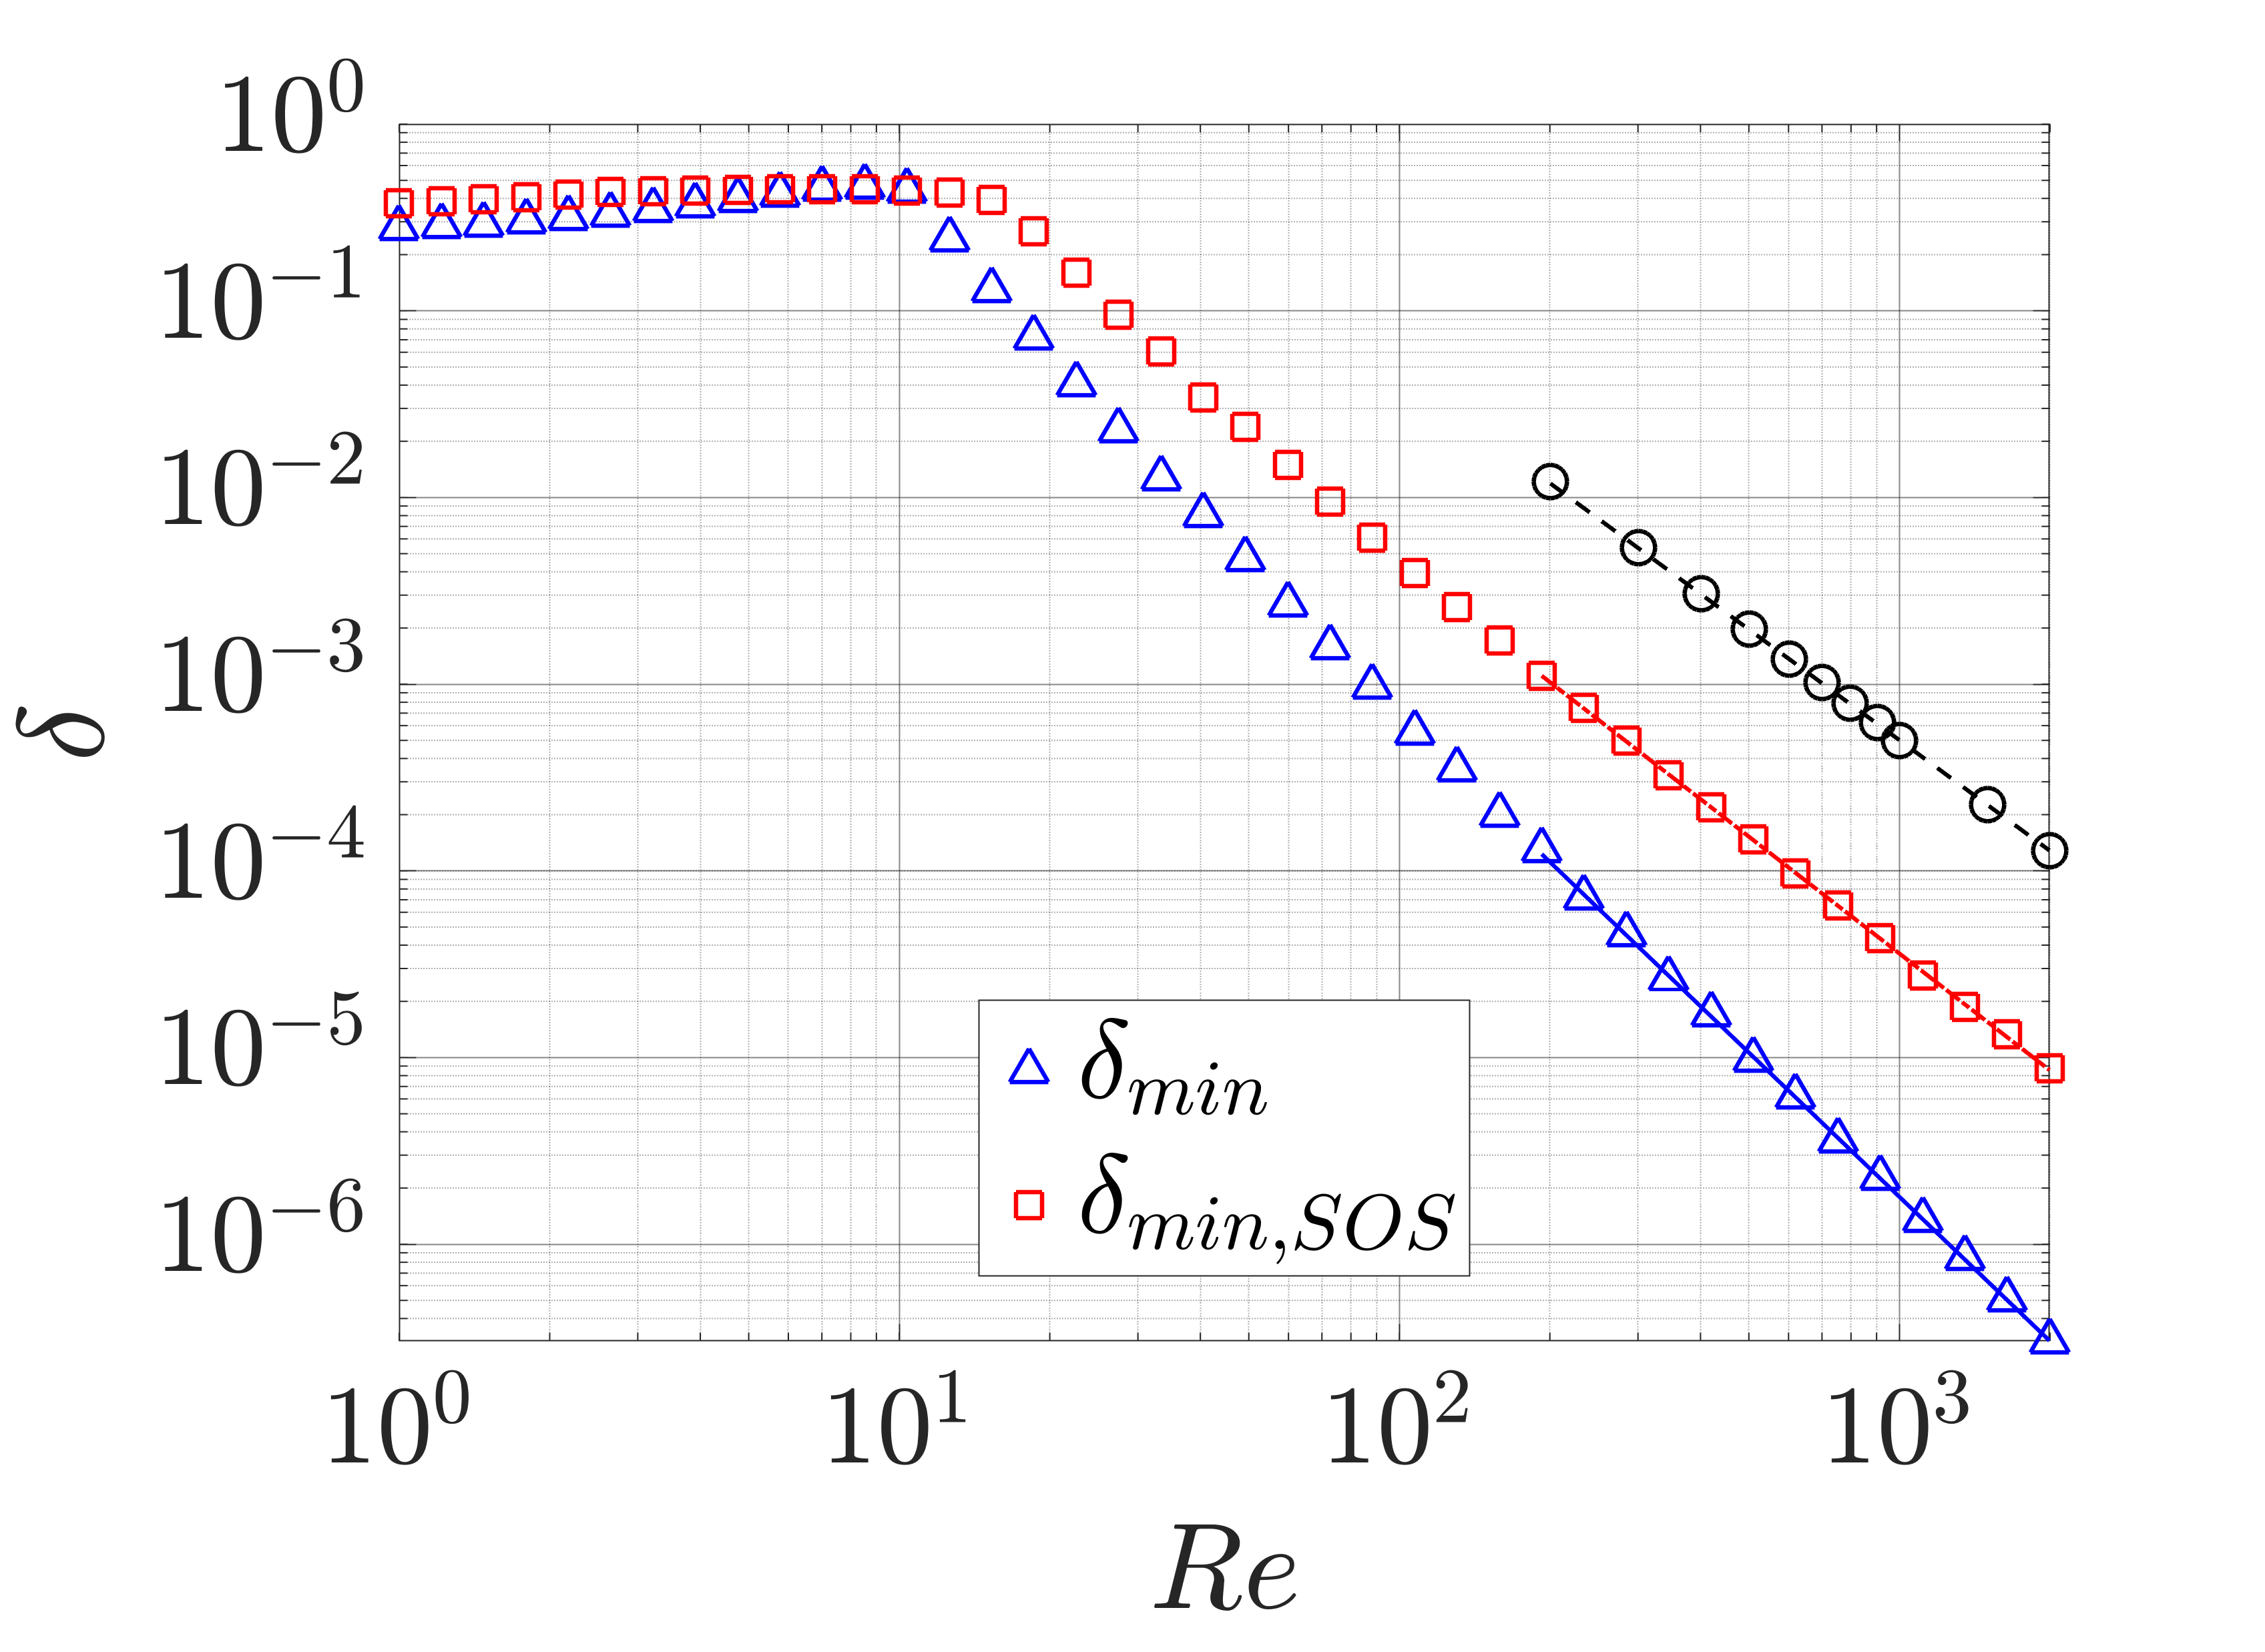
\includegraphics[width=2in]{ROA_9D_GalerkinNS_4pi2pi_sostools_eps8_40lmi_lmi_ROA_delta_min_com.png}
\captionof{figure}{The blue triangles are $\delta_{\text{min}}$ with the blue solid line as $\delta_{\text{min}}=10^{1.95}Re^{-2.57}$. The red rectangles are $\delta_{\text{min,SOS}}$ with the red dash-dot line as $\delta_{\text{min,SOS}}=10^{1.80}Re^{-2.08}$. The black circles are the minimum distance $d_{\text{min}}$ with the black dashed line $d_{\text{min}}=10^{2.61}Re^{-1.97}$ below in which all trajectories converge to the laminar state obtained from simulations \citep{Joglekar2015}.}
\label{fig:delta_min}
\end{minipage}
 \begin{minipage}[c]{0.49\textwidth}
    \centering
\begin{tabular}[b]{ccc}
    \toprule    %[0.3pt] 
Method  & LMI & SOS \\
    \midrule    %[0.3pt]
% \noalign{\smallskip}
 Formulation time (s) & 195 & 731253\\
      SDP Solver time (s) & 683 & 18578\\
      Size of the largest PSD cone & 18 & 54\\
      Number of constraints & 74 & 795\\
    \bottomrule %[0.3pt]
\end{tabular}
\captionof{table}{Comparison of requested computational resoures between the proposed LMI framework in equation (\ref{eq:LMI}) and SOS approach.}
\label{tab:time_compare}
\end{minipage}



\vspace{-2mm}
\section{APPLICATION TO SHEAR FLOW MODELS}
\vspace{-2mm}



Here, we consider a nine-dimensional Galerkin model \citep{Moehlis2004} for sinusoidal shear flows to demonstrate the proposed method. The resulting critical perturbation amplitude $\delta_{\text{min}}$ is shown in figure \ref{fig:delta_min} as the blue triangles, and it shows a power law $\delta_{\text{min}}=10^{1.95}Re^{-2.57}$ as Reynolds number varies. In figure \ref{fig:delta_min}, the $d_{\text{min}}$ in the black circles also shows a power law $10^{2.61}Re^{-1.97}$ below in which all trajectories converges to the laminar state identified from 10,000 randomly chosen initial conditions \citep{Joglekar2015} using the same sinusoidal shear flow model. The critical amplitude $\delta_{\text{min}}$ identified using this framework is conservative, but \emph{any} trajectories starting from inside $||\boldsymbol{a}||_2\leq \delta_{\text{min}}$ are guaranteed to converge to the laminar state. The critical perturbation amplitude obtained using the current input-output inspired method may be further improved through the Sum of Squares (SOS) approach \citep{papachristodoulou2013sostools}, which will automatically explore the property of the nonlinear term at the expense of more computational resources. The resulting $\delta_{\text{min,SOS}}$ is shown in figure \ref{fig:delta_min} as the red rectangle with a power law $\delta_{\text{min,SOS}}=10^{1.80}Re^{-2.08}$. Here, we note the results obtained from the SOS are closer to the simulation results compared with the previous employed linear matrix inequality framework, but the SOS approach request more computational resources as show in Table \ref{tab:time_compare}. 




\vspace{-2mm}
\section{CONCLUSIONS}
\vspace{-2mm}


This work constructs an input-output inspired model of the nonlinear term that is constrained by system physics to be energy conserving and have bounded input-output energy in a local region. These constraints allow us to determine the permissible level of perturbation amplitude to maintain a laminar flow state in a computationally efficient manner. We apply our approach to low dimensional nonlinear shear flow models \citep{Moehlis2004} for a range of Reynolds numbers. The results from our analytically derived bounds are consistent with the bounds identified through exhaustive simulations. However, our results are obtained at a much lower computational cost and have the benefit of providing a provable guarantee that a certain level of perturbation is permissible. The results obtained from the current framework may be further improved through employing some prevailing nonlinear approaches such as Sum of Squares (SOS) programming at the expense of computational cost.



% \begin{thebibliography}{9}
% \bibitem{Ref1}
% Goulart, P. J., & Chernyshenko, S. Global stability analysis of fluid flows using sum-of-squares. \textit{Physica D}, \textbf{241}(6), 692-704, 2012.
% \bibitem{Ref2}
% Joglekar, M., Feudel, U., & Yorke, J. A. Geometry of the edge of chaos in a low-dimensional turbulent shear flow model. \textit{Phys. Rev. E}, \textbf{91}(5), 052903, 2015.
% \bibitem{Ref3}
% Joseph, D. D. Stability of fluid motions I (Vol. 27). Springer Science & Business Media, 2013.
% \bibitem{Ref4}
% Löfberg, J.. "YALMIP: A toolbox for modeling and optimization in MATLAB." Proceedings of the CACSD Conference. Vol. 3. 2004.
% \bibitem{Ref5}
% Moehlis, J., Faisst, H., & Eckhardt, B. A low-dimensional model for turbulent shear flows. \textit{New Journal of Physics}, \textbf{6}(1), 56, 2004.
% \end{thebibliography}
\vspace{-5mm}
\setlength{\bibsep}{-0pt}
\renewcommand\bibpreamble{\vspace{-1\baselineskip}} % choose a suitable vert. skip
{\footnotesize\bibliography{main}}

\bibliographystyle{abbrvnat}


\end{document}
